\documentclass{article}
\usepackage{graphicx}
\usepackage{listings}
\usepackage{xcolor}

\definecolor{codegray}{gray}{0.9}
\lstdefinestyle{mystyle}{
    backgroundcolor=\color{codegray},
    basicstyle=\ttfamily,
    frame=single,
    breaklines=true
}
\lstset{style=mystyle}

\newcommand{\class}{}

\begin{document}

\title{Footprinting and Reconnaissance Experiment: Using Google for Company Information}
\author{Priyanshu Kumar Sharma, 2022-B-17102004A, B.Tech CTIS, SEM-VI/B}
\date{\today}
\maketitle

\section{Objective}
To gather publicly available information about a company using Google search techniques.

\section{Steps to Perform the Experiment}

\subsection{Step 1: Define Your Target Company}
\begin{itemize}
    \item Choose a company you want to investigate.
    \item Make sure your search is legal and ethical, following all privacy guidelines.
\end{itemize}

\subsection{Step 2: Perform Basic Google Searches}
\textbf{Command:}
\begin{lstlisting}
www.oracle.com/in/
\end{lstlisting}
\textbf{BAT Script:}
\begin{lstlisting}
@echo off
start https://www.google.com/search?q=www.oracle.com/in/
\end{lstlisting}
\textbf{Description:} This searches for general information about www.oracle.com/in/.
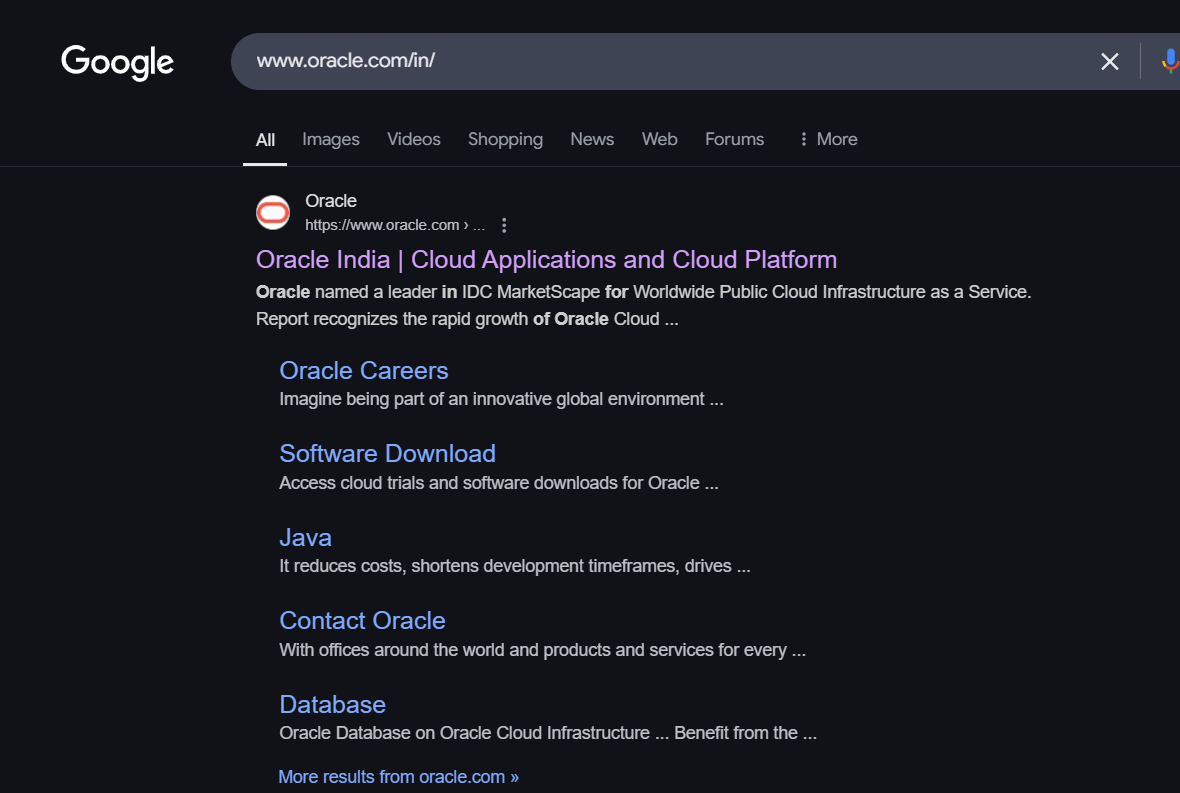
\includegraphics[width=0.8\textwidth]{images/basic_search.png}

\subsection{Step 3: Use Advanced Google Search Operators}
\textbf{Find the company's official website:}
\begin{lstlisting}
site:www.oracle.com/in/
\end{lstlisting}
\textbf{BAT Script:}
\begin{lstlisting}
@echo off
start https://www.google.com/search?q=site:www.oracle.com/in/
\end{lstlisting}
\textbf{Description:} Filters results to only show pages from the official website.
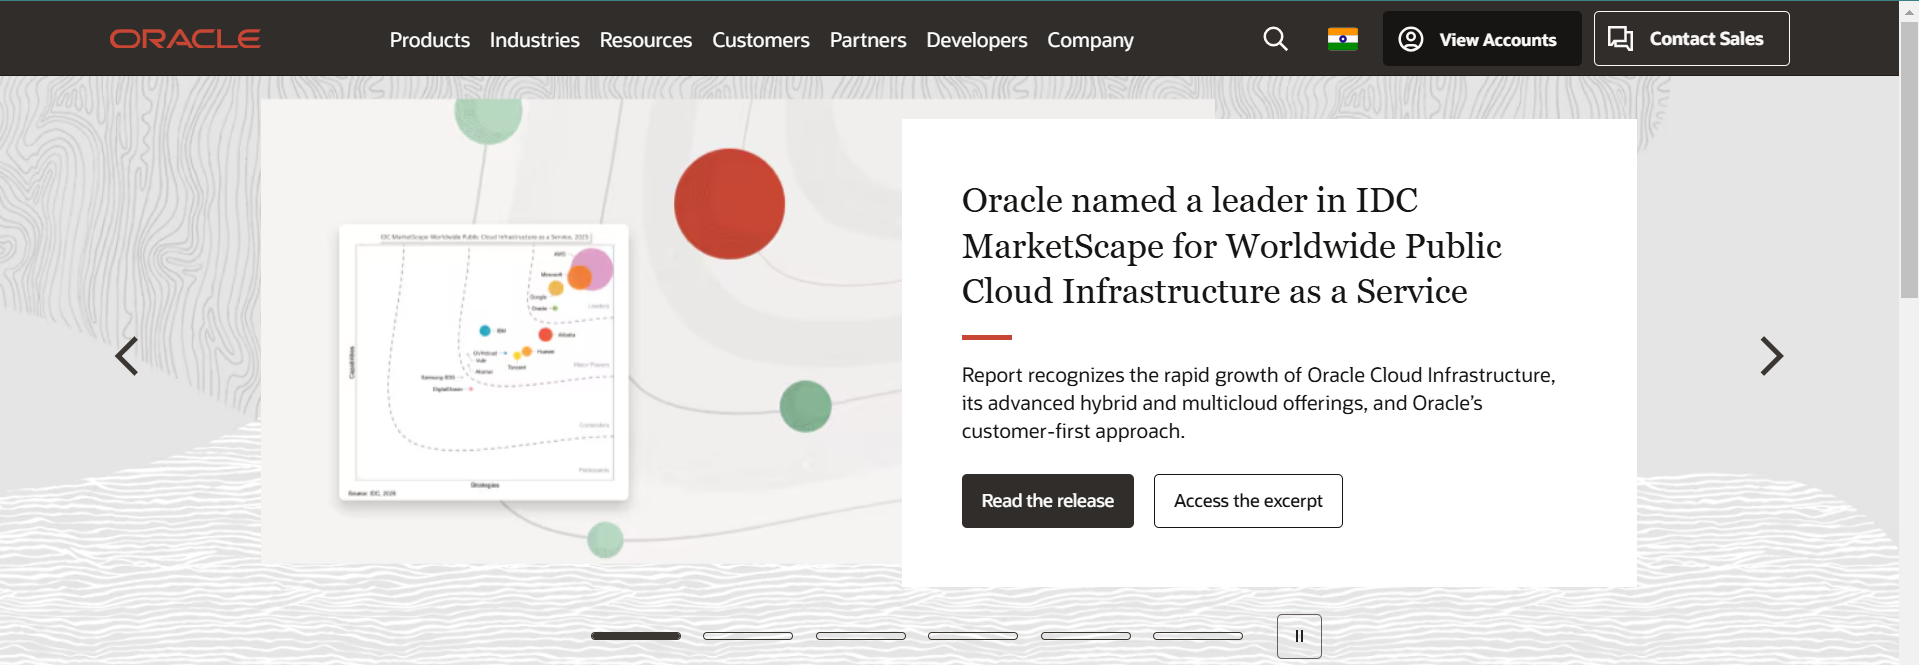
\includegraphics[width=0.8\textwidth]{images/official_website.png}

\textbf{Find specific file types (e.g., PDFs, Docs, XLSX):}
\begin{lstlisting}
site:www.oracle.com/in/ filetype:pdf
\end{lstlisting}
\textbf{BAT Script:}
\begin{lstlisting}
@echo off
start https://www.google.com/search?q=site:www.oracle.com/in/+filetype:pdf
\end{lstlisting}
\textbf{Description:} Finds publicly available PDF files from the official website.
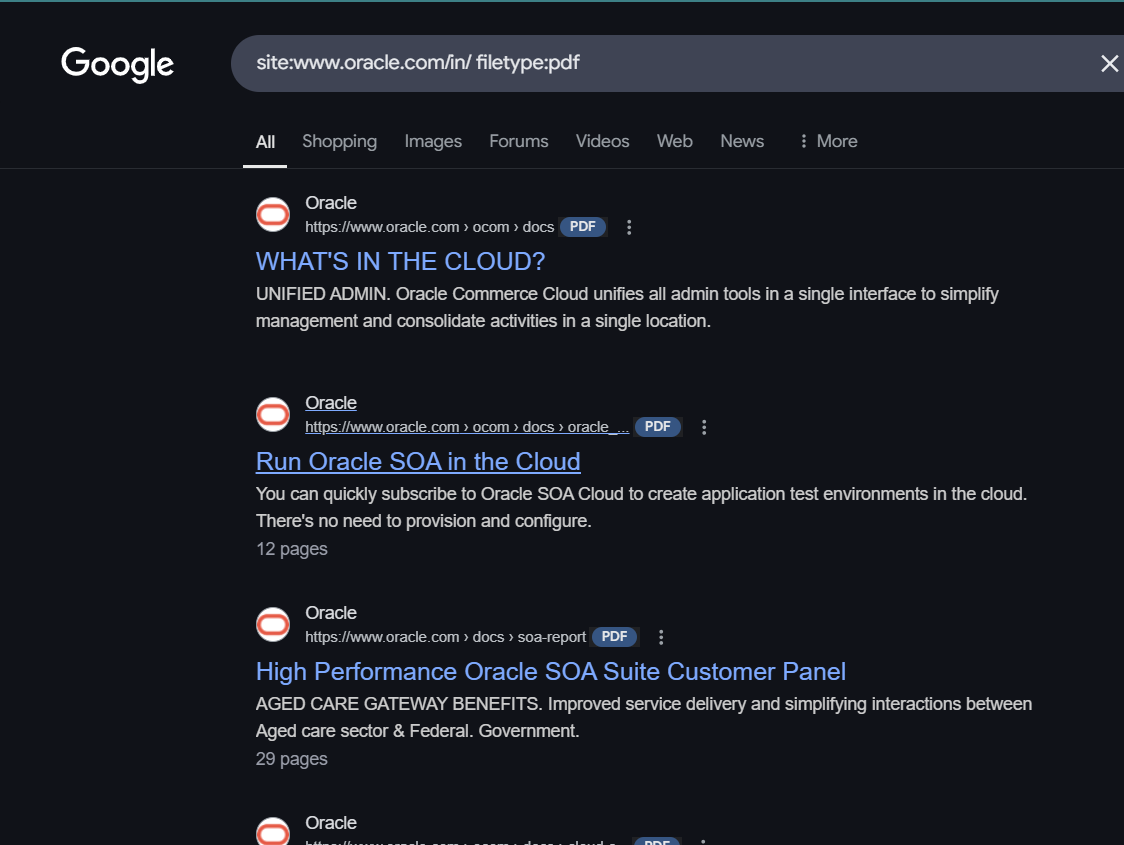
\includegraphics[width=1.0\textwidth]{images/filetype_search.png}

\textbf{Find sensitive directories or subdomains:}
\begin{lstlisting}
site:www.oracle.com/in/ inurl:admin
site:www.oracle.com/in/ inurl:login
\end{lstlisting}
\textbf{BAT Script:}
\begin{lstlisting}
@echo off
start https://www.google.com/search?q=site:www.oracle.com/in/+inurl:admin
start https://www.google.com/search?q=site:www.oracle.com/in/+inurl:login
\end{lstlisting}
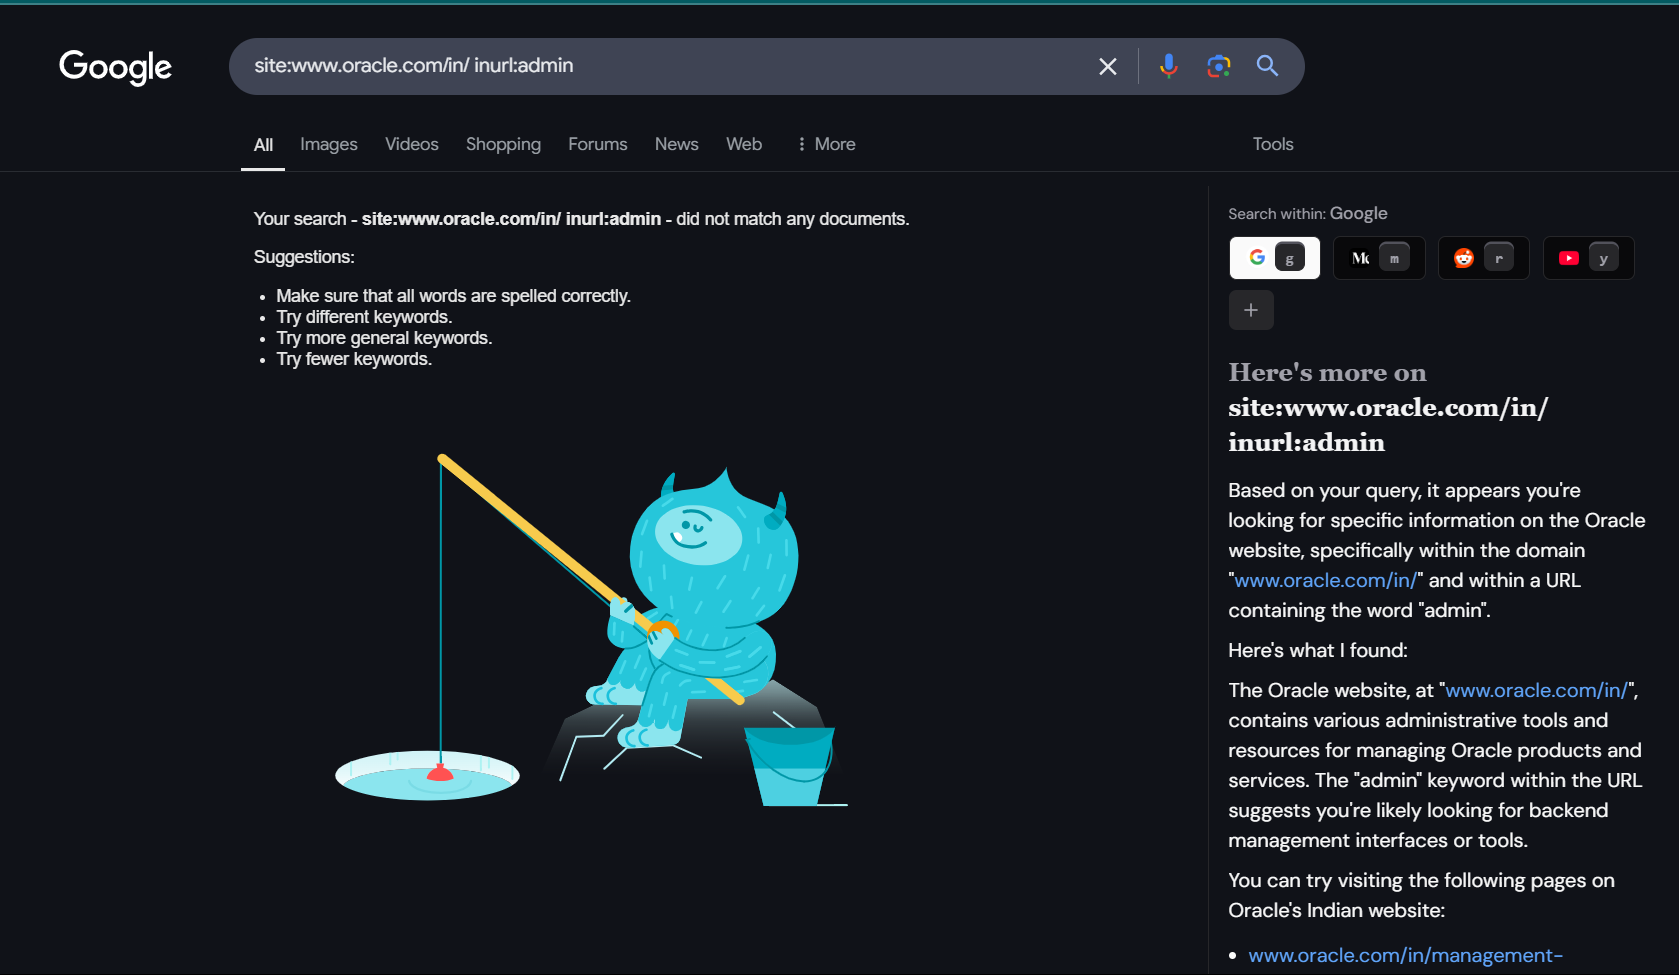
\includegraphics[width=0.8\textwidth]{images/sensitive_dirs.png}
\newline
\textbf{Description:} Helps discover administrative and login pages.

\textbf{Discover employee names and emails:}
\begin{lstlisting}
"@www.oracle.com/in/"
\end{lstlisting}
\textbf{BAT Script:}
\begin{lstlisting}
@echo off
start https://www.google.com/search?q=%22@www.oracle.com/in/%22
\end{lstlisting}
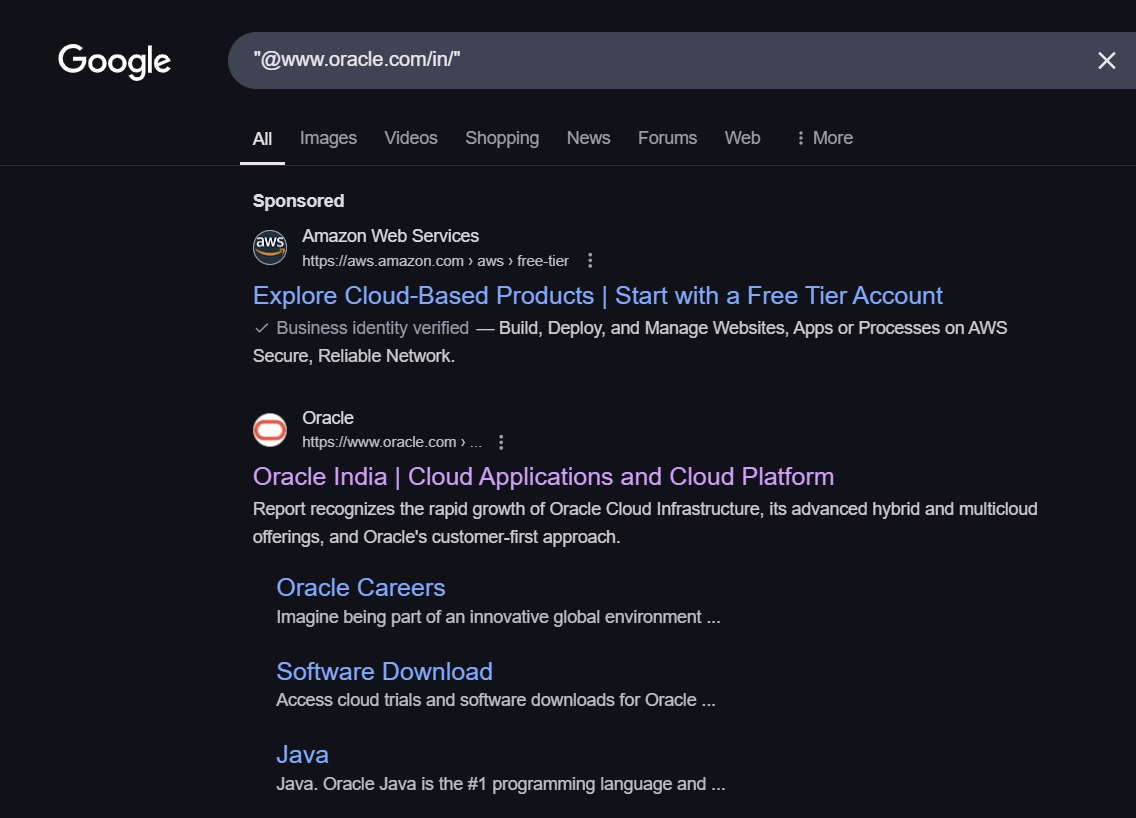
\includegraphics[width=0.8\textwidth]{images/email_search.png}
\textbf{Description:} Searches for publicly listed emails associated with the company.

\newpage
\section{Google Dorking for Social Media}
\subsection{Gather Social Media Information}
\textbf{Find social media presence:}
\begin{lstlisting}
www.oracle.com/in/ site:linkedin.com
www.oracle.com/in/ site:twitter.com
www.oracle.com/in/ site:facebook.com
\end{lstlisting}
\textbf{BAT Script:}
\begin{lstlisting}
@echo off
start https://www.google.com/search?q=www.oracle.com/in/+site:linkedin.com
start https://www.google.com/search?q=www.oracle.com/in/+site:twitter.com
start https://www.google.com/search?q=www.oracle.com/in/+site:facebook.com
\end{lstlisting}
includegraphics[width=0.8\textwidth]{social_media.png}
\newline
\textbf{Description:} Helps locate the company's social media accounts.
\

\subsection{Use Google Dorking for Deeper Insights}
\textbf{Find internal documents:}
\begin{lstlisting}
site:www.oracle.com/in/ confidential
\end{lstlisting}
\textbf{BAT Script:}
\begin{lstlisting}
@echo off
start https://www.google.com/search?q=site:www.oracle.com/in/+confidential
\end{lstlisting}
\textbf{Description:} Searches for confidential documents.
\includegraphics[width=0.8\textwidth]{confidential_docs.png}

\textbf{Find exposed directories:}
\begin{lstlisting}
intitle:"index of" "parent directory" site:www.oracle.com/in/
\end{lstlisting}
\textbf{BAT Script:}
\begin{lstlisting}
@echo off
start https://www.google.com/search?q=intitle:%22index+of%22+%22parent+directory%22+site:www.oracle.com/in/
\end{lstlisting}
\textbf{Description:} Identifies open directory listings.
\includegraphics[width=0.8\textwidth]{open_dirs.png}

\textbf{Find possible vulnerabilities:}
\begin{lstlisting}
site:www.oracle.com/in/ "Error 404" OR "SQL syntax error"
\end{lstlisting}
\textbf{BAT Script:}
\begin{lstlisting}
@echo off
start https://www.google.com/search?q=site:www.oracle.com/in/+%22Error+404%22+OR+%22SQL+syntax+error%22
\end{lstlisting}
\textbf{Description:} Checks for errors that might indicate security vulnerabilities.
\includegraphics[width=0.8\textwidth]{vulnerabilities.png}

\subsection{Summarize Findings}
\begin{itemize}
    \item Company address, contact details
    \item Publicly available documents (PDFs, reports, whitepapers)
    \item Employee names and job roles
    \item Possible security vulnerabilities (if any)
\end{itemize}

\section{Precautions \& Ethical Considerations}
\begin{itemize}
    \item Only use publicly available data.
    \item Do not attempt to bypass security measures.
    \item Do not engage in illegal activities (hacking, phishing, etc.).
    \item Respect privacy and data protection laws.
\end{itemize}

\end{document}
